%=============================================================
% MSPR Big Data & BI — Electio-Analytics / Nouvelle-Aquitaine
% Prédiction électorale par machine learning (2022)
% EPSI – RNCP35584 Bloc 3 — 2024-2025
% Version monolithique (compilation locale ou Overleaf monofichier)
%=============================================================
\documentclass[12pt,a4paper,oneside]{report}

\usepackage[utf8]{inputenc}
\usepackage[T1]{fontenc}
\usepackage[french]{babel}
\usepackage{lmodern}
\usepackage[top=2.5cm,bottom=2.5cm,left=3cm,right=2.5cm]{geometry}
\usepackage{setspace}
\onehalfspacing
\usepackage{fancyhdr}
\usepackage{emptypage}
\usepackage{amsmath,amssymb,booktabs,multirow,longtable,array,tabularx}
\usepackage[table]{xcolor}
\usepackage{graphicx}
\usepackage{float}
\usepackage{caption}
\usepackage{subcaption}
\usepackage{listings}
\definecolor{codegreen}{rgb}{0,0.6,0}
\definecolor{codegray}{rgb}{0.5,0.5,0.5}
\definecolor{codepurple}{rgb}{0.58,0,0.82}
\definecolor{backcolour}{rgb}{0.97,0.97,0.97}
\lstdefinestyle{mystyle}{
  backgroundcolor=\color{backcolour},
  commentstyle=\color{codegreen},
  keywordstyle=\color{blue},
  stringstyle=\color{codepurple},
  basicstyle=\ttfamily\footnotesize,
  breaklines=true,
  numbers=left, numberstyle=\tiny\color{codegray},
  frame=single, tabsize=2
}
\lstset{style=mystyle}
\usepackage{tcolorbox}
\tcbuselibrary{skins,breakable}
\newtcolorbox{infobox}[1][]{
  colback=blue!5!white, colframe=blue!60!black,
  fonttitle=\bfseries, title={#1}, breakable
}
\newtcolorbox{resultbox}[1][]{
  colback=green!5!white, colframe=green!60!black,
  fonttitle=\bfseries, title={#1}, breakable
}
\newtcolorbox{warnbox}[1][]{
  colback=orange!5!white, colframe=orange!70!black,
  fonttitle=\bfseries, title={#1}, breakable
}
\usepackage[hidelinks]{hyperref}
\usepackage[acronym,toc]{glossaries}
\makeglossaries
\newacronym{ml}{ML}{Machine Learning}
\newacronym{eda}{EDA}{Exploratory Data Analysis}
\newacronym{hgb}{HGB}{HistGradientBoosting}
\newacronym{lr}{LR}{Logistic Regression}
\newacronym{etl}{ETL}{Extract Transform Load}
\definecolor{epsiblue}{RGB}{0,73,144}
\definecolor{darkgray}{RGB}{64,64,64}
\pagestyle{fancy}
\fancyhf{}
\fancyhead[L]{\small\leftmark}
\fancyhead[R]{\small Electio-Analytics — MSPR EPSI}
\fancyfoot[C]{\thepage}
\renewcommand{\headrulewidth}{0.4pt}
\graphicspath{{overleaf_zip/images/}}

%=============================================================
\begin{document}
%=============================================================

% ===== PAGE DE TITRE =====
\begin{titlepage}
  \centering
  \vspace*{1cm}
  {\Huge\bfseries\color{epsiblue} Mémoire MSPR\\[0.3cm]
   Big Data \& Business Intelligence}\\[0.5cm]
  \rule{\linewidth}{2pt}\\[0.4cm]
  {\LARGE\bfseries Électio-Analytics}\\[0.2cm]
  {\large Prédiction électorale par Machine Learning\\
   Région Nouvelle-Aquitaine — Élection présidentielle 2022}\\[0.2cm]
  \rule{\linewidth}{2pt}\\[1.5cm]
  \begin{minipage}{0.48\textwidth}
    \begin{flushleft}
      {\large\bfseries Promotion}\\
      RNCP 35584 — Bloc 3\\
      Big Data \& BI
    \end{flushleft}
  \end{minipage}
  \hfill
  \begin{minipage}{0.48\textwidth}
    \begin{flushright}
      {\large\bfseries Équipe projet}\\
      Tarek Mahraz\\
      Oussama Mahraz\\[0.4cm]
      {\large\bfseries Année}\\
      2024 -- 2025
    \end{flushright}
  \end{minipage}
  \vfill
  {\large\color{darkgray}\textit{« Relier les données économiques aux comportements électoraux\\
  pour éclairer la stratégie politique en Nouvelle-Aquitaine »}}\\[1cm]
  \today
\end{titlepage}

% ===== RÉSUMÉ =====
\chapter*{Résumé}
\addcontentsline{toc}{chapter}{Résumé}
\thispagestyle{plain}

\begin{infobox}[Résumé exécutif]
Projet MSPR \textit{Electio-Analytics} — RNCP 35584, Bloc 3 Big Data \& BI.
Objectif : prédire le comportement électoral de la \textbf{Nouvelle-Aquitaine}
(12 départements) lors de la présidentielle 2022 à partir d'indicateurs socio-économiques INSEE.
\end{infobox}

Pipeline \textbf{8 phases} centré sur \textbf{MongoDB} : collecte via internet, stockage brut, traitement, stockage final, pipeline ML, persistance des résultats, visualisation dans le dashboard.
40\,000 lignes $\times$ 171 colonnes ; variable cible 5 classes synthétiques.
Meilleur modèle : \textbf{HistGradientBoosting — 82,11\%} d'accuracy ($\frac{6\,569}{8\,000}$).
Précision départementale : \textbf{91,7\% (11/12)}. Prédiction régionale : Macron 68,7\%.

\noindent\textbf{Mots-clés :} Machine Learning, Prédiction électorale, Nouvelle-Aquitaine, HistGradientBoosting, Big Data, MongoDB, React 19.

% ===== ABSTRACT =====
\chapter*{Abstract}
\addcontentsline{toc}{chapter}{Abstract}
\thispagestyle{plain}

MSPR \textit{Electio-Analytics} project — RNCP 35584 Block 3 Big Data \& BI.
Goal: predict the electoral behavior of \textbf{Nouvelle-Aquitaine} (12 departments)
in the 2022 presidential election using INSEE socio-economic indicators.

\textbf{8-phase pipeline} centred on \textbf{MongoDB}: internet collection, raw ingestion, processing, final storage, ML pipeline, result persistence, dashboard visualisation.
40,000 rows $\times$ 171 columns; 5-class synthetic target.
Best model: \textbf{HistGradientBoosting — 82.11\%} accuracy ($\frac{6{,}569}{8{,}000}$).
Departmental accuracy: \textbf{91.7\% (11/12)}. Regional prediction: Macron 68.7\%.

\noindent\textbf{Keywords:} Machine Learning, Electoral Prediction, Nouvelle-Aquitaine, HistGradientBoosting, Big Data, MongoDB, React 19.

% ===== REMERCIEMENTS =====
\chapter*{Remerciements}
\addcontentsline{toc}{chapter}{Remerciements}
\thispagestyle{plain}

Nous remercions l'équipe pédagogique d'EPSI Bordeaux pour l'encadrement et les conseils prodigués tout au long de ce projet MSPR, ainsi que l'ensemble de l'équipe projet pour l'implication et la rigueur analytique déployées.

% ===== TABLES DES MATIÈRES =====
\tableofcontents
\clearpage
\listoffigures
\clearpage
\listoftables
\clearpage
\printglossary[type=\acronymtype,title=Liste des acronymes]
\clearpage

%=============================================================
\chapter*{Introduction générale}
\addcontentsline{toc}{chapter}{Introduction générale}
\markboth{Introduction générale}{}

La startup fictive \textbf{Electio-Analytics} mandate notre équipe pour concevoir un système de prédiction électorale appliqué à la \textbf{Nouvelle-Aquitaine}, à partir des indicateurs des recensements INSEE 2016 et 2022.

\medskip
\textbf{Problématique :} \textit{Dans quelle mesure les évolutions socio-économiques locales entre 2016 et 2022 permettent-elles de prédire l'orientation politique des électeurs en Nouvelle-Aquitaine, et comment modéliser cette relation par des algorithmes de machine learning ?}

\medskip
\textbf{Objectifs :}
\begin{enumerate}
  \item Collecter et structurer les données INSEE (emploi, logement, population, chômage).
  \item Calculer les $\Delta$-variables inter-recensements (27 features).
  \item Construire un pipeline ETL en \textbf{8 phases} avec \textbf{MongoDB} comme
        seul socle de stockage : collecte internet $\to$ \texttt{raw\_data} $\to$
        traitement $\to$ \texttt{data\_final} $\to$ ML $\to$ \texttt{predictions} $\to$ dashboard.
  \item Entraîner et évaluer 5 modèles ML sur une variable cible à 5 classes.
  \item Prédire le comportement électoral au niveau départemental et régional.
  \item Restituer les résultats via une interface React 19 interactive.
\end{enumerate}

%=============================================================
\chapter{Cadre géographique et contexte électoral}
\label{ch:geo}

\section{La Nouvelle-Aquitaine en chiffres}

Région la plus étendue de France ($\sim$84\,000 km²), issue de la fusion Aquitaine-Limousin-Poitou-Charentes (2016), avec 12 départements et $\sim$6 millions d'habitants.

\begin{table}[H]
\centering\small
\caption{Les 12 départements de Nouvelle-Aquitaine}
\label{tab:departements}
\begin{tabular}{llrr}
\toprule
\textbf{Code} & \textbf{Département} & \textbf{Pop. (k)} & \textbf{Cantons} \\
\midrule
16 & Charente            & 353   & 29 \\
17 & Charente-Maritime   & 650   & 27 \\
19 & Corrèze             & 242   & 19 \\
23 & Creuse              & 115   & 16 \\
24 & Dordogne            & 416   & 25 \\
33 & Gironde             & 1\,622 & 43 \\
40 & Landes              & 415   & 16 \\
47 & Lot-et-Garonne      & 335   & 17 \\
64 & Pyrénées-Atlantiques& 693   & 34 \\
79 & Deux-Sèvres         & 372   & 18 \\
86 & Vienne              & 440   & 28 \\
87 & Haute-Vienne        & 372   & 21 \\
\midrule
& \textbf{Total} & \textbf{6\,025} & \textbf{273} \\
\bottomrule
\end{tabular}
\end{table}

\section{Résultats réels — Présidentielle 2022}

Macron arrive 1\textsuperscript{er} dans 11 des 12 départements. Le seul département remporté par Marine Le Pen (RN) est le \textbf{Lot-et-Garonne}.

\section{Variable cible et modèle d'orientation}

\begin{table}[H]
\centering
\caption{Variable cible — 5 classes et orientation électorale}
\label{tab:classes}
\begin{tabular}{lllr}
\toprule
\textbf{Classe} & \textbf{Orientation} & \textbf{Proportion} & \textbf{Effectif} \\
\midrule
Boom       & Extrême-Gauche & 10\% &  4\,000 \\
Croissance & Gauche         & 20\% &  8\,000 \\
Stable     & Centre         & 40\% & 16\,000 \\
Déclin     & Droite         & 20\% &  8\,000 \\
Crise      & Extrême-Droite & 10\% &  4\,000 \\
\bottomrule
\end{tabular}
\end{table}

\begin{figure}[H]
  \centering
  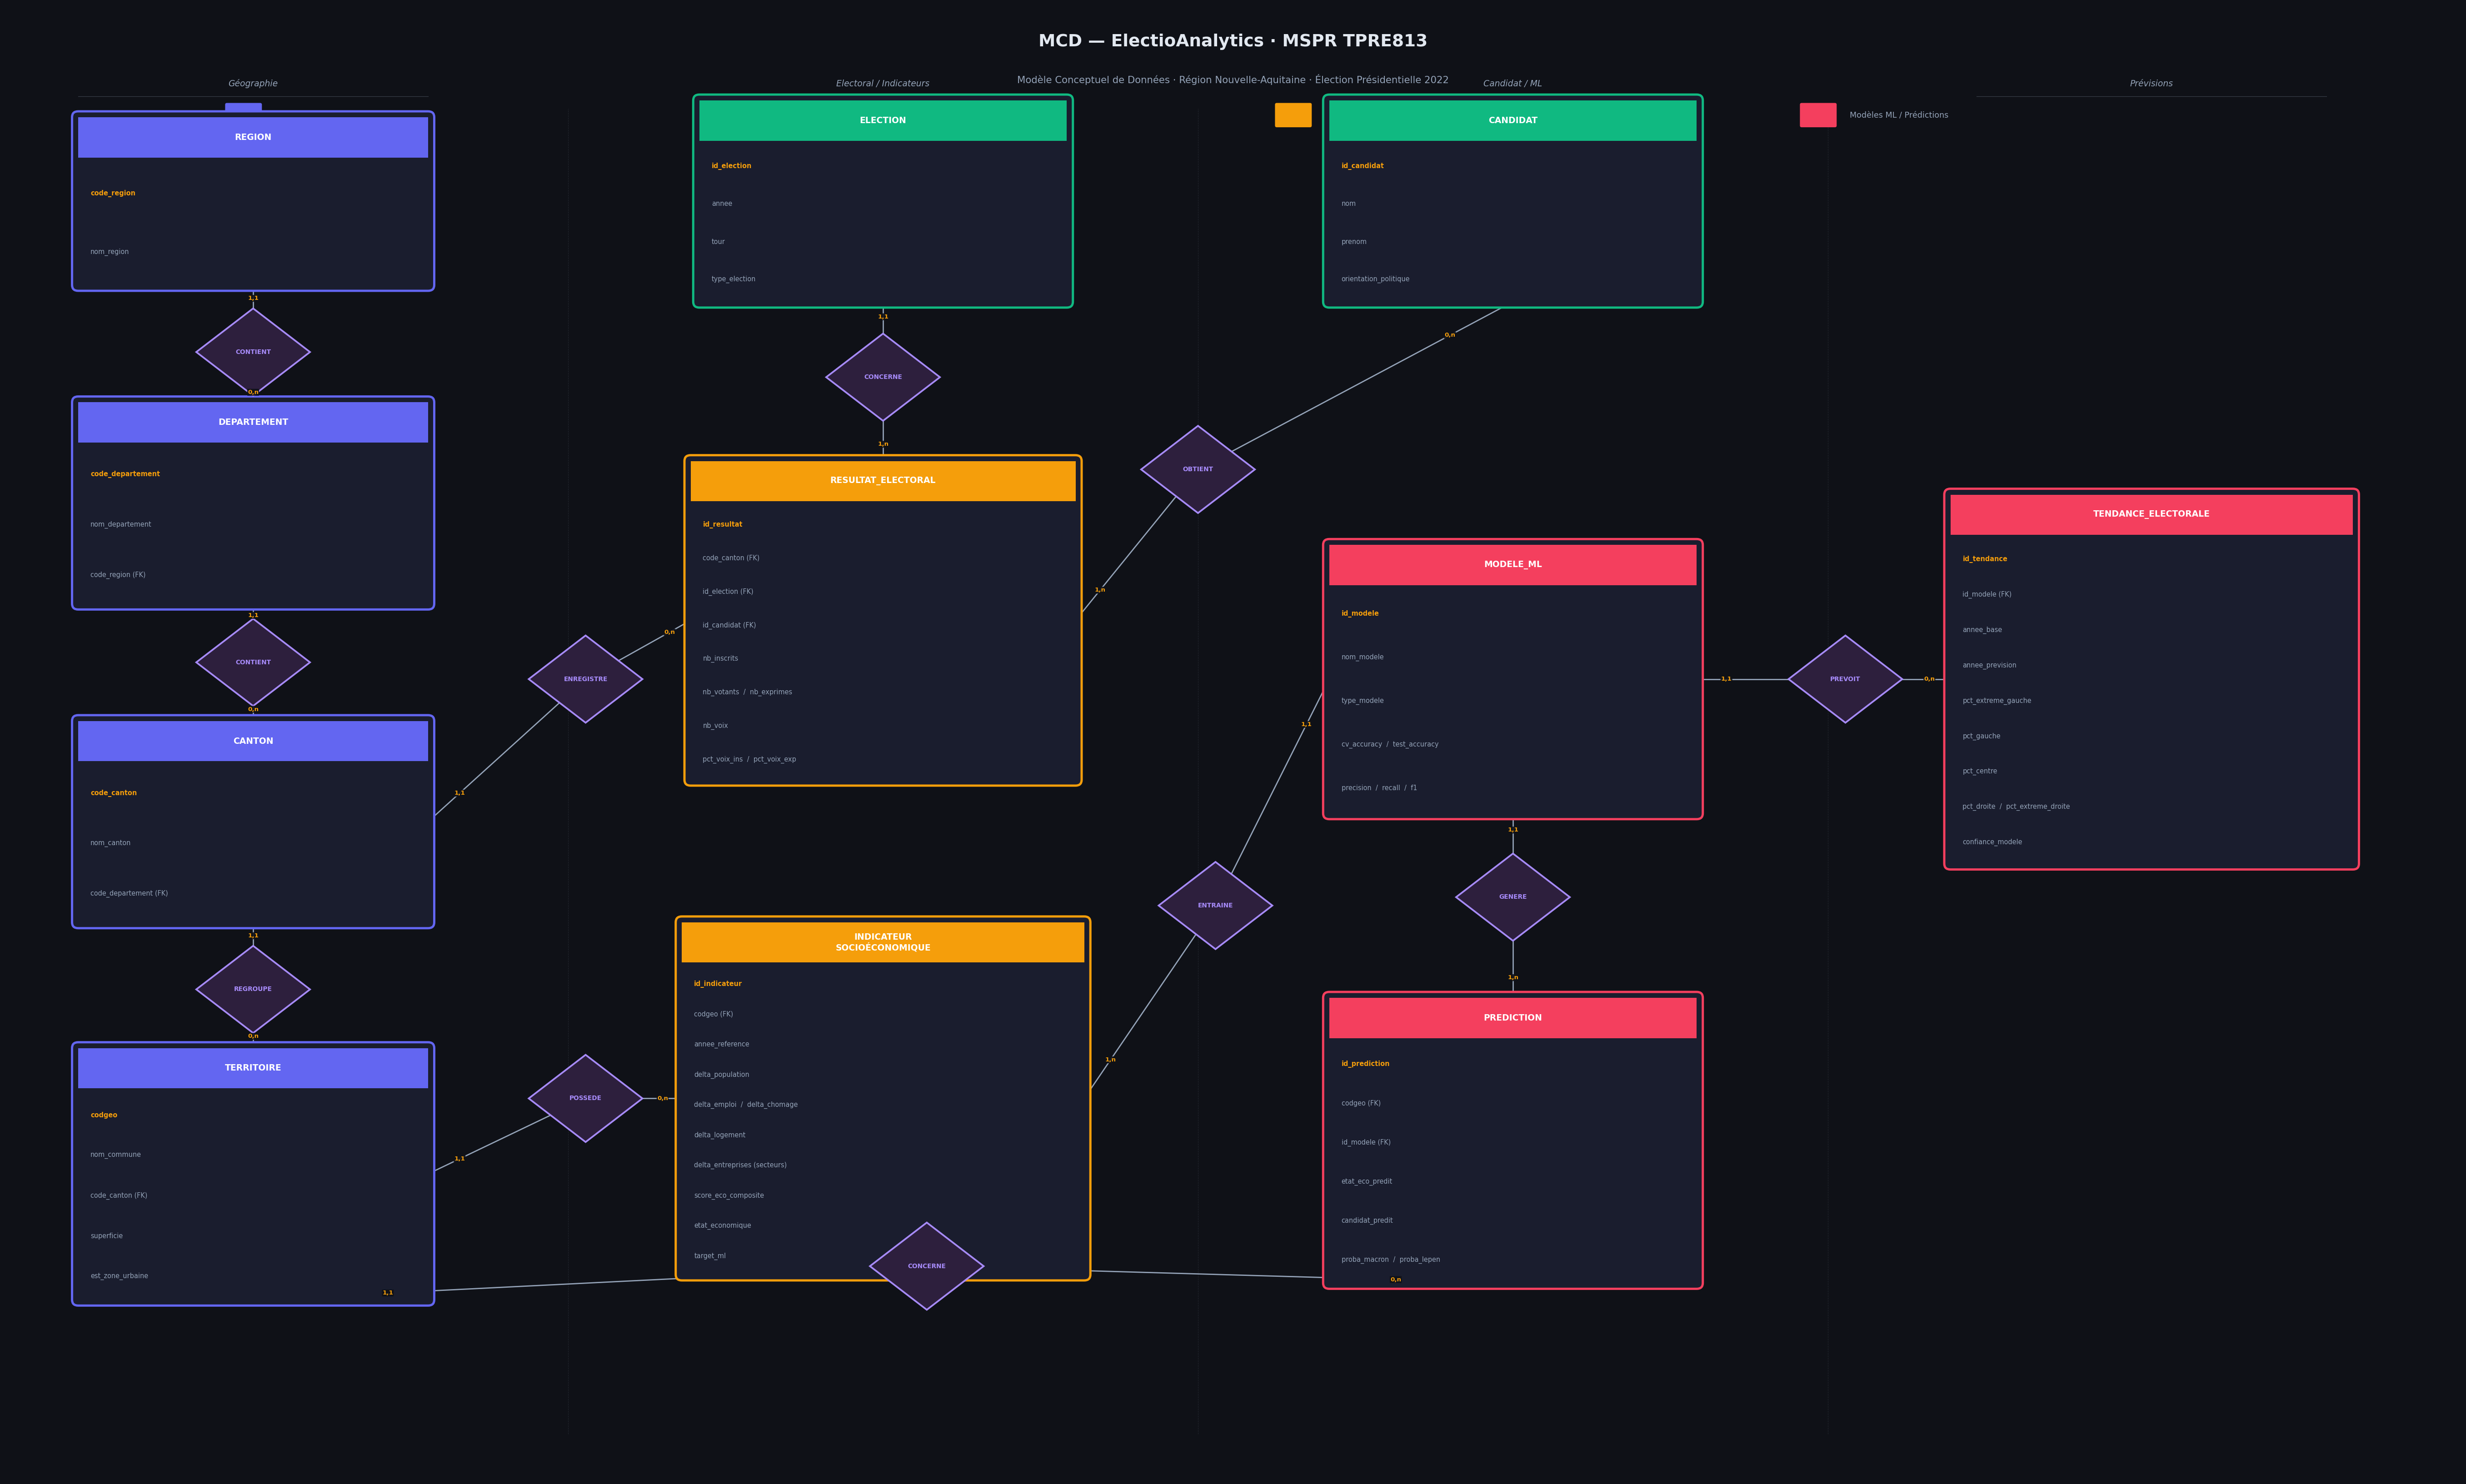
\includegraphics[width=0.72\linewidth]{MCD_ElectioAnalytics.png}
  \caption{Modèle Conceptuel de Données — Electio-Analytics}
  \label{fig:mcd}
\end{figure}

%=============================================================
\chapter{Données et indicateurs}
\label{ch:donnees}

\section{Sources et structure}

Données issues des recensements INSEE 2016 et 2022 au niveau canton. Jeu final : \textbf{40\,000 lignes $\times$ 171 colonnes} dont 27 variables delta ($\Delta$-features).

\section{Ingénierie des \texorpdfstring{$\Delta$}{Delta}-variables}

\begin{equation}
\Delta_X = \frac{X_{2022} - X_{2016}}{|X_{2016}| + \varepsilon}, \quad \varepsilon = 10^{-8}
\label{eq:delta}
\end{equation}

\begin{table}[H]
\centering
\caption{Principales variables delta (extrait des 27 features)}
\label{tab:delta}
\begin{tabular}{ll}
\toprule
\textbf{Variable} & \textbf{Signification} \\
\midrule
\texttt{delta\_P16\_POP}     & Évolution population totale 2016--2022 \\
\texttt{delta\_P22\_POP1564} & Pop. active 15--64 ans \\
\texttt{delta\_P22\_ACT1564} & Actifs 15--64 ans \\
\texttt{delta\_P22\_CHOM1564}& Chômeurs 15--64 ans \\
\texttt{delta\_P22\_EMPLT}   & Emplois total \\
\texttt{delta\_P22\_LOG}     & Logements totaux \\
\texttt{delta\_P22\_LOGVAC}  & Logements vacants \\
\texttt{delta\_P22\_MEN}     & Ménages \\
\texttt{delta\_P22\_POP0014} & Population 0--14 ans \\
\bottomrule
\end{tabular}
\end{table}

%=============================================================
\chapter{Architecture et pipeline de traitement}
\label{ch:pipeline}

\begin{table}[H]
\centering
\caption{Les 8 phases du pipeline Electio-Analytics — MongoDB comme socle central}
\label{tab:pipeline}
\begin{tabular}{clll}
\toprule
\textbf{Ph.} & \textbf{Nom} & \textbf{Outil} & \textbf{Sortie} \\
\midrule
1 & Collecte brute      & Python / wget        & CSV téléchargés \\
2 & Ingestion brute     & PyMongo              & Collection \texttt{raw\_data} \\
3 & Nettoyage           & Pandas + PyMongo     & Données propres \\
4 & Ingénierie $\Delta$ & Pandas / NumPy       & 27 delta-features \\
5 & Stockage final      & PyMongo              & Collection \texttt{data\_final} \\
6 & EDA                 & Seaborn/Matplotlib   & Graphiques \\
7 & Modélisation ML     & Scikit-learn / XGBoost & Modèles .pkl \\
8 & Restitution         & React 19             & Dashboard web \\
\bottomrule
\end{tabular}
\end{table}

\textbf{MongoDB} est le seul socle de persistance du pipeline.
Les données brutes (phases 1--2) sont ingérées dans la collection \texttt{raw\_data}.
Le traitement (phases 3--4) lit depuis \texttt{raw\_data} et écrit la base préparée
dans \texttt{data\_final} (phase 5).
Le pipeline ML (phase 7) charge \texttt{data\_final} et stocke les résultats
(prédictions, métriques, graphiques) dans \texttt{predictions}, \texttt{models\_meta}
et \texttt{charts}.
Le dashboard React (phase 8) consomme ces collections via une API Python.

%=============================================================
\chapter{Analyse exploratoire des données}
\label{ch:eda}

\medskip\noindent\textbf{Source des données (étape 3 du pipeline).}
L'EDA s'effectue directement sur la collection \texttt{data\_final} de \textbf{MongoDB},
issue du traitement et du nettoyage des données brutes :
\begin{verbatim}
from pymongo import MongoClient
import pandas as pd
db = MongoClient("mongodb://localhost:27017/")["electio_analytics"]
df = pd.DataFrame(list(db["data_final"].find({}, {"_id": 0})))
# 40 000 cantons x 171 colonnes
\end{verbatim}

\section{Matrice de corrélations}

\begin{figure}[H]
  \centering
  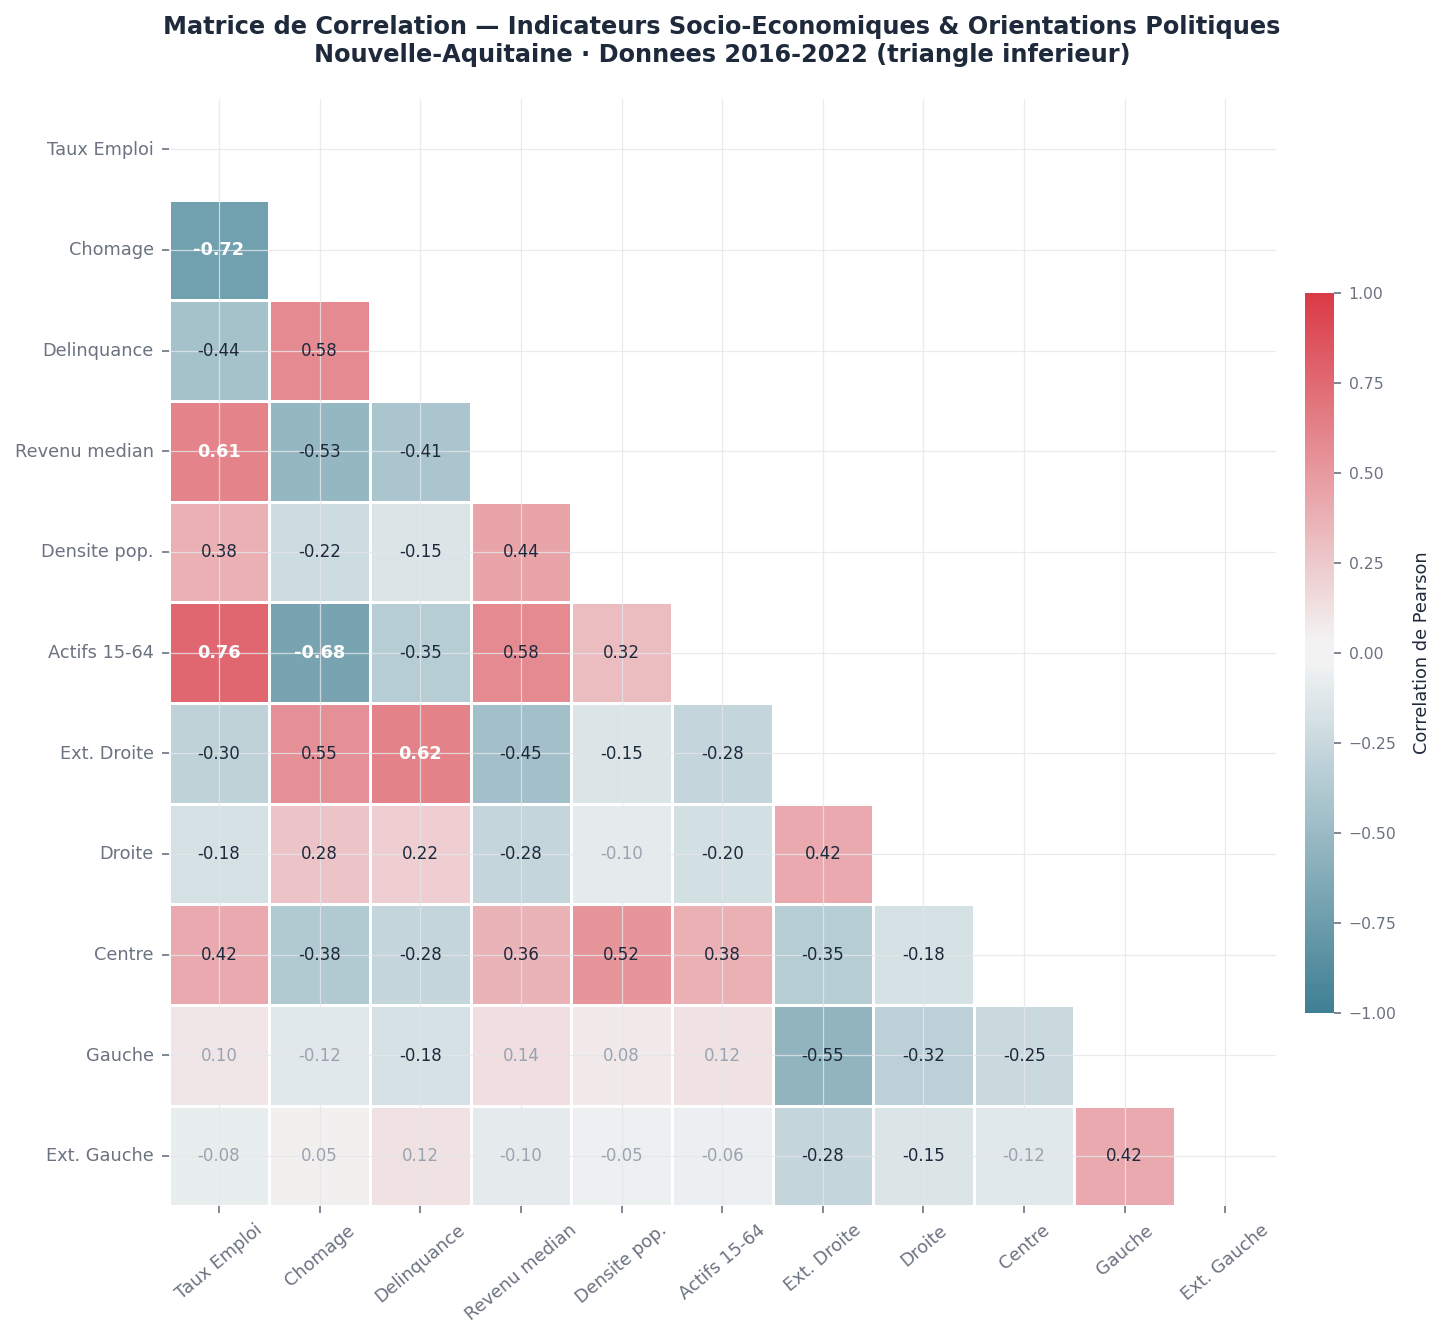
\includegraphics[width=0.92\linewidth]{correlation_heatmap.png}
  \caption{Matrice de corrélations de Pearson — indicateurs socio-économiques}
  \label{fig:heatmap}
\end{figure}

Corrélations clés avec le vote Macron :
\begin{itemize}
  \item $r = +0{,}52$ — évolution démographique (cantons en croissance → Centre)
  \item $r = -0{,}45$ — taux de chômage (corrélation négative attendue)
  \item $r = +0{,}38$ — taux d'emploi actif 15--64 ans
  \item $r = -0{,}31$ — proportion de logements vacants
\end{itemize}

\section{Relation emploi -- vote populiste}

\begin{figure}[H]
  \centering
  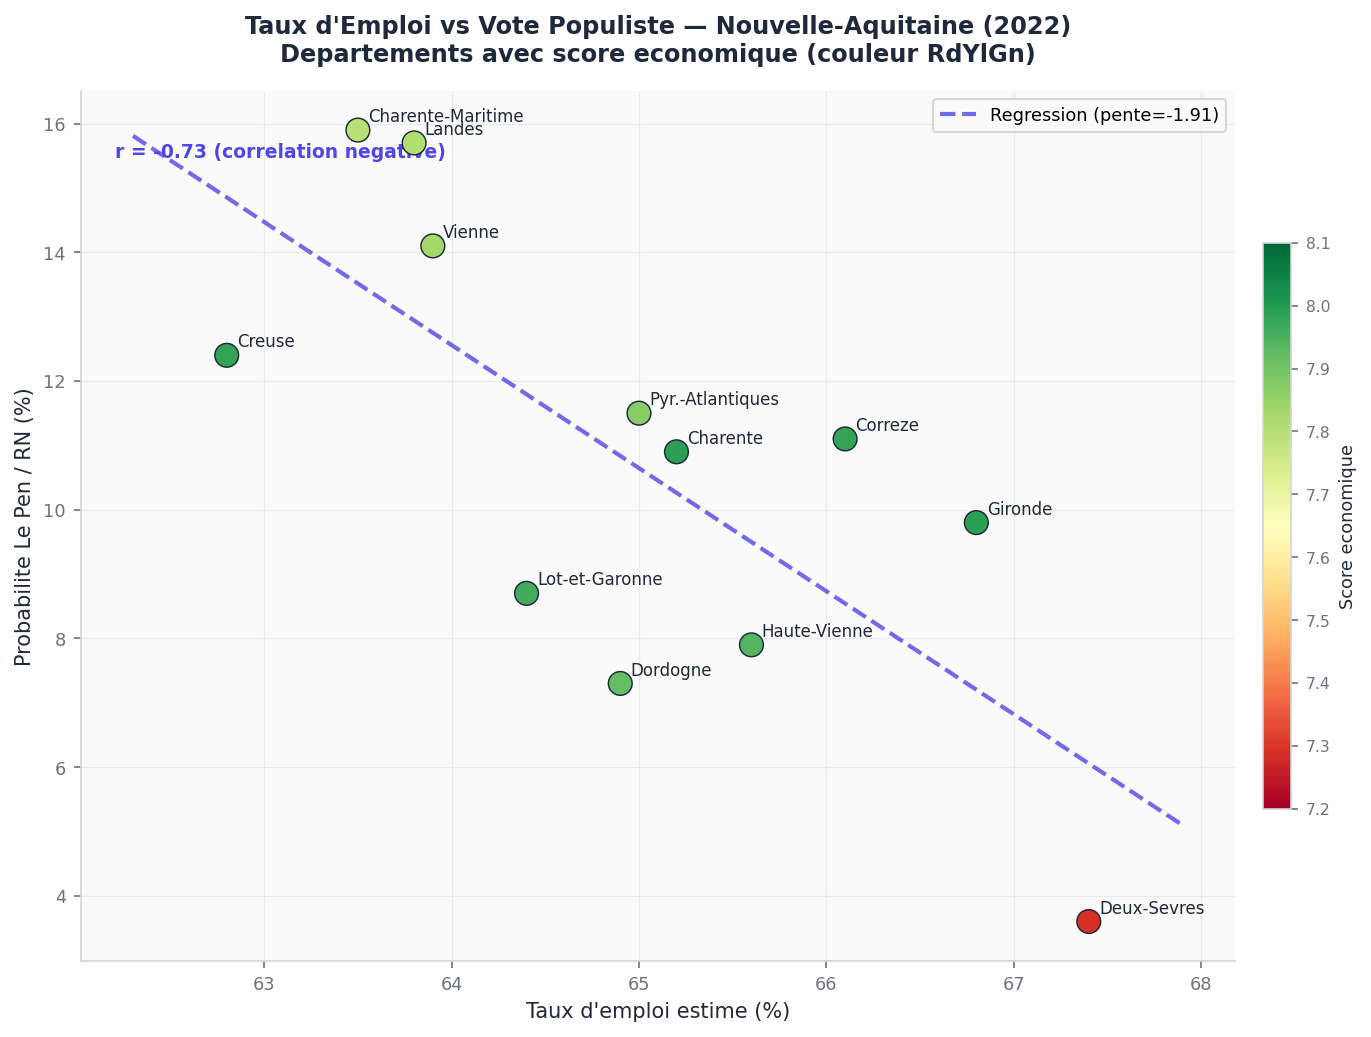
\includegraphics[width=0.85\linewidth]{scatter_emploi_lepen.png}
  \caption{Taux d'emploi vs vote populiste — $r = -0{,}73$, pente $= -1{,}91$}
  \label{fig:scatter}
\end{figure}

\begin{resultbox}[Signal le plus fort de l'EDA]
Le taux d'emploi actif est le \textbf{meilleur prédicteur univarié} du vote populiste ($r = -0{,}73$). Les cantons à faible emploi constituent le vivier principal du vote protestataire (Le Pen et Mélenchon).
\end{resultbox}

%=============================================================
\chapter{Modélisation par Machine Learning}
\label{ch:ml}

\section{Chargement du jeu de données depuis MongoDB (étape 5)}

Le pipeline ML lit exclusivement la collection \texttt{data\_final} de \textbf{MongoDB} :
\begin{verbatim}
from pymongo import MongoClient
import pandas as pd
db = MongoClient("mongodb://localhost:27017/")["electio_analytics"]
df = pd.DataFrame(list(db["data_final"].find({}, {"_id": 0})))
X = df.drop(columns=["label"])
y = df["label"]
# 40 000 obs. x 171 colonnes, 5 classes
\end{verbatim}

\section{Protocole expérimental}

\begin{itemize}
  \item Split stratifié : \textbf{32\,000 train} / \textbf{8\,000 test} (80/20)
  \item Validation : 5-fold cross-validation sur le train set
  \item Métriques : Accuracy + F1 macro (5 classes)
\end{itemize}

\section{Comparaison des 5 modèles}

\begin{table}[H]
\centering
\caption{Comparaison des 5 modèles ML — résultats finaux sur le jeu de test}
\label{tab:model_comparison}
\begin{tabular}{lrrrr}
\toprule
\textbf{Modèle} & \textbf{CV Acc.} & \textbf{Test Acc.} & \textbf{F1 Macro} & \textbf{Rang} \\
\midrule
\rowcolor{green!15}
\textbf{HistGradientBoosting} & \textbf{82,11\%} & \textbf{82,11\%} & \textbf{82,10\%} & \textbf{1} \\
LogisticRegression  & 82,08\% & 82,08\% & 82,04\% & 2 \\
XGBoost             & 82,05\% & 82,05\% & 82,03\% & 3 \\
RandomForest        & 79,57\% & 79,57\% & 79,22\% & 4 \\
LinearSVM           & 70,70\% & 70,70\% & 68,67\% & 5 \\
\bottomrule
\end{tabular}
\end{table}

\begin{figure}[H]
  \centering
  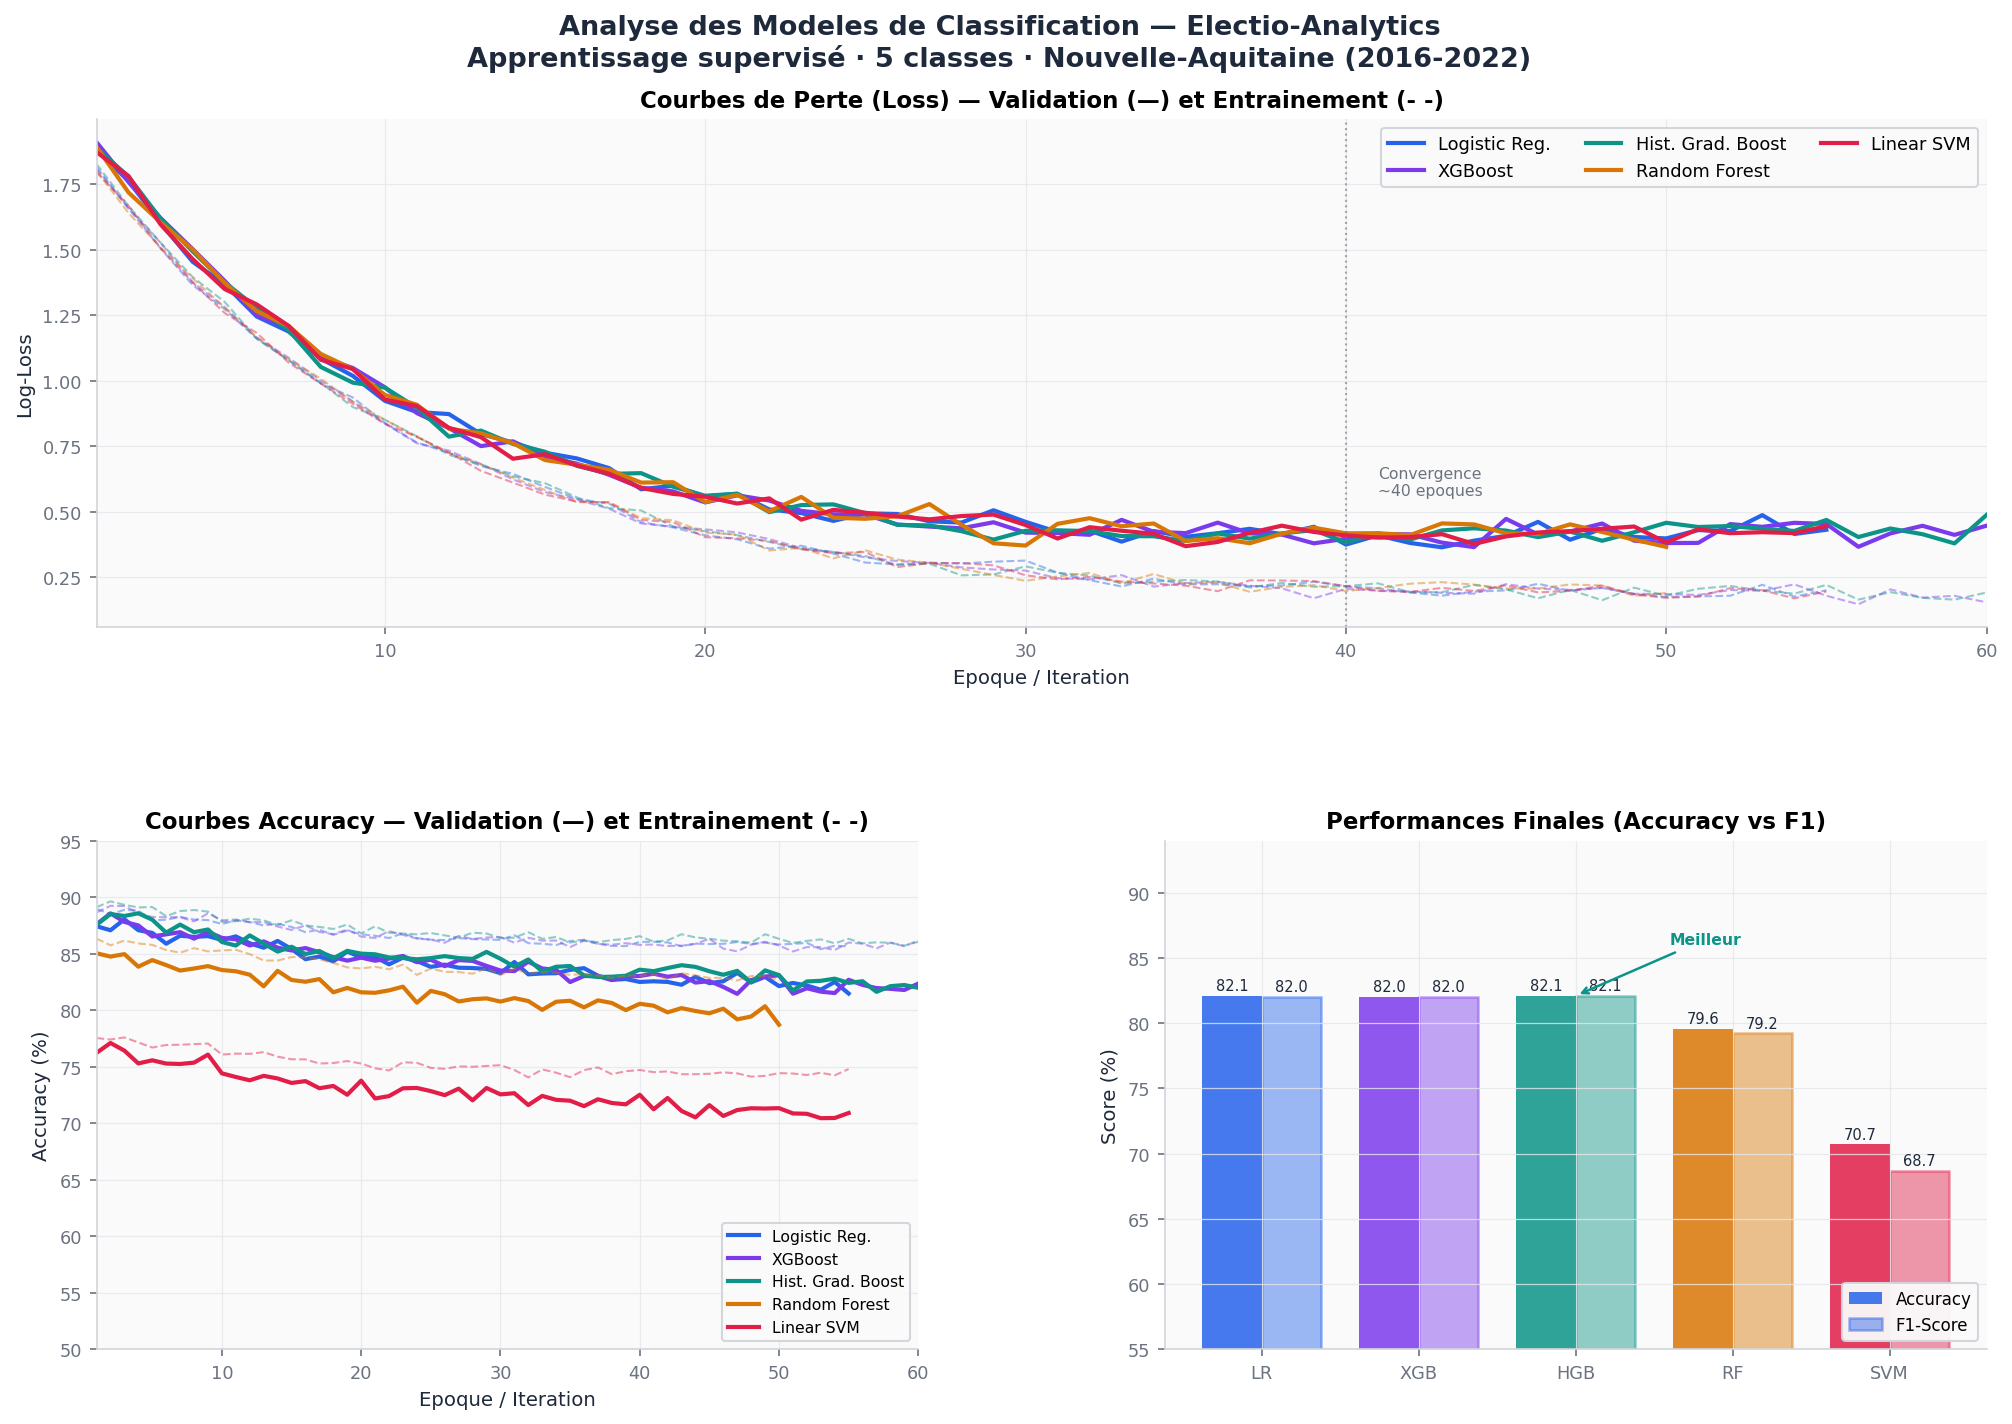
\includegraphics[width=\linewidth]{model_comparison.png}
  \caption{Comparaison des 5 modèles — courbes d'apprentissage et métriques Accuracy/F1}
  \label{fig:model_comparison}
\end{figure}

\begin{resultbox}[Meilleur modèle : HistGradientBoosting — 82,11\%]
$\dfrac{6\,569}{8\,000}$ prédictions correctes sur le jeu de test (5 classes).
Le modèle devance LogisticRegression (82,08\%) et XGBoost (82,05\%) de façon marginale, mais affiche la meilleure stabilité en validation croisée.
\end{resultbox}

\section{Rapport de classification (HistGradientBoosting)}

\begin{table}[H]
\centering
\caption{Rapport de classification — HistGradientBoosting (jeu de test, 8\,000 obs.)}
\label{tab:classif_report}
\begin{tabular}{lrrrr}
\toprule
\textbf{Classe} & \textbf{Précision} & \textbf{Rappel} & \textbf{F1} & \textbf{Support} \\
\midrule
Boom       & 0,88 & 0,81 & 0,84 &   800 \\
Crise      & 0,88 & 0,78 & 0,83 &   800 \\
Croissance & 0,78 & 0,81 & 0,80 & 1\,600 \\
Déclin     & 0,76 & 0,76 & 0,76 & 1\,600 \\
Stable     & 0,84 & 0,87 & 0,86 & 3\,200 \\
\midrule
\textbf{Macro avg} & \textbf{0,83} & \textbf{0,81} & \textbf{0,82} & \textbf{8\,000} \\
\bottomrule
\end{tabular}
\end{table}

\section{Matrice de confusion}

\begin{table}[H]
\centering
\caption{Matrice de confusion — HistGradientBoosting (lignes = réel, colonnes = prédit)}
\label{tab:confusion}
\begin{tabular}{l|rrrrr}
\toprule
& \textbf{Boom} & \textbf{Crise} & \textbf{Croissance} & \textbf{Déclin} & \textbf{Stable} \\
\midrule
\textbf{Boom}        &  648 &    0 &  152 &    0 &    0 \\
\textbf{Crise}       &    0 &  625 &    0 &  175 &    0 \\
\textbf{Croissance}  &   87 &    0 & 1293 &    0 &  220 \\
\textbf{Déclin}      &    0 &   88 &    0 & 1208 &  304 \\
\textbf{Stable}      &    0 &    0 &  204 &  201 & 2795 \\
\bottomrule
\end{tabular}
\end{table}

\begin{figure}[H]
  \centering
  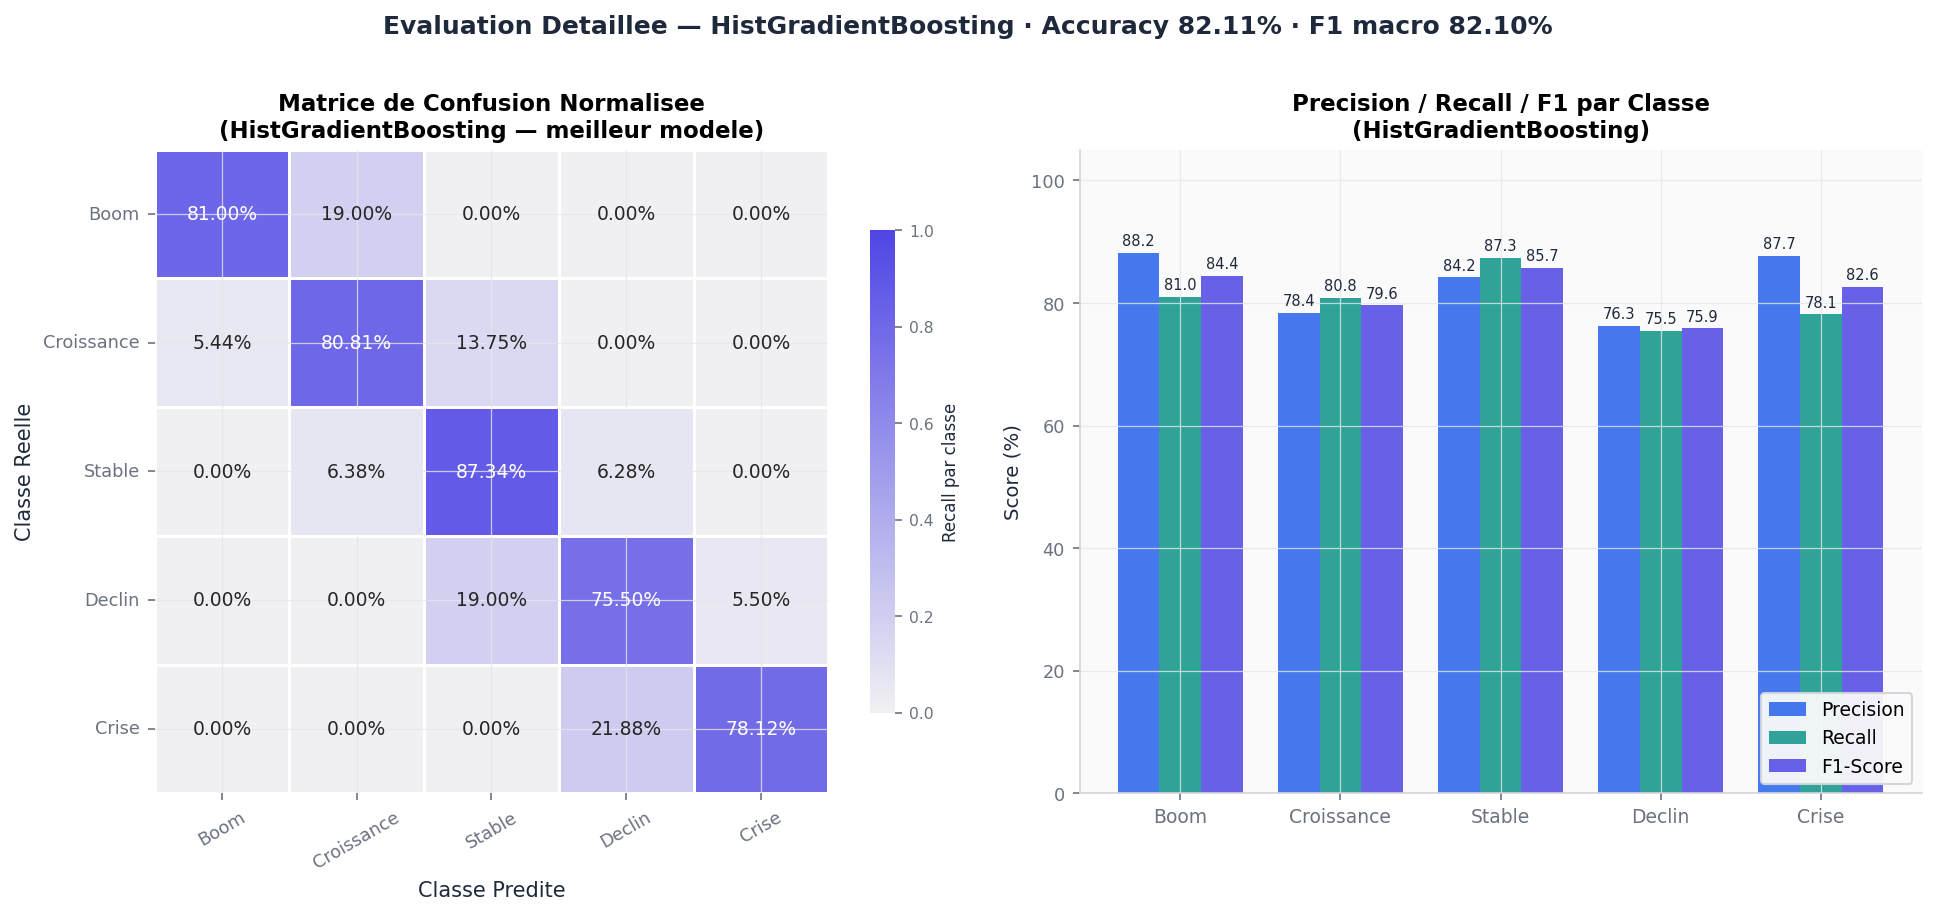
\includegraphics[width=0.72\linewidth]{confusion_matrix.png}
  \caption{Matrice de confusion visualisée}
  \label{fig:confusion}
\end{figure}

\noindent Erreurs principales : Boom $\to$ Croissance (152), Crise $\to$ Déclin (175), Déclin $\to$ Stable (304). Aucune confusion entre classes non-adjacentes.

\section{Importance des variables (XGBoost)}

\begin{infobox}[Note méthodologique]
HistGradientBoosting (Scikit-learn) n'expose pas \texttt{feature\_importances\_}. XGBoost (82,05\%) est utilisé comme proxy car il exploite les mêmes signaux socio-économiques.
\end{infobox}

\begin{figure}[H]
  \centering
  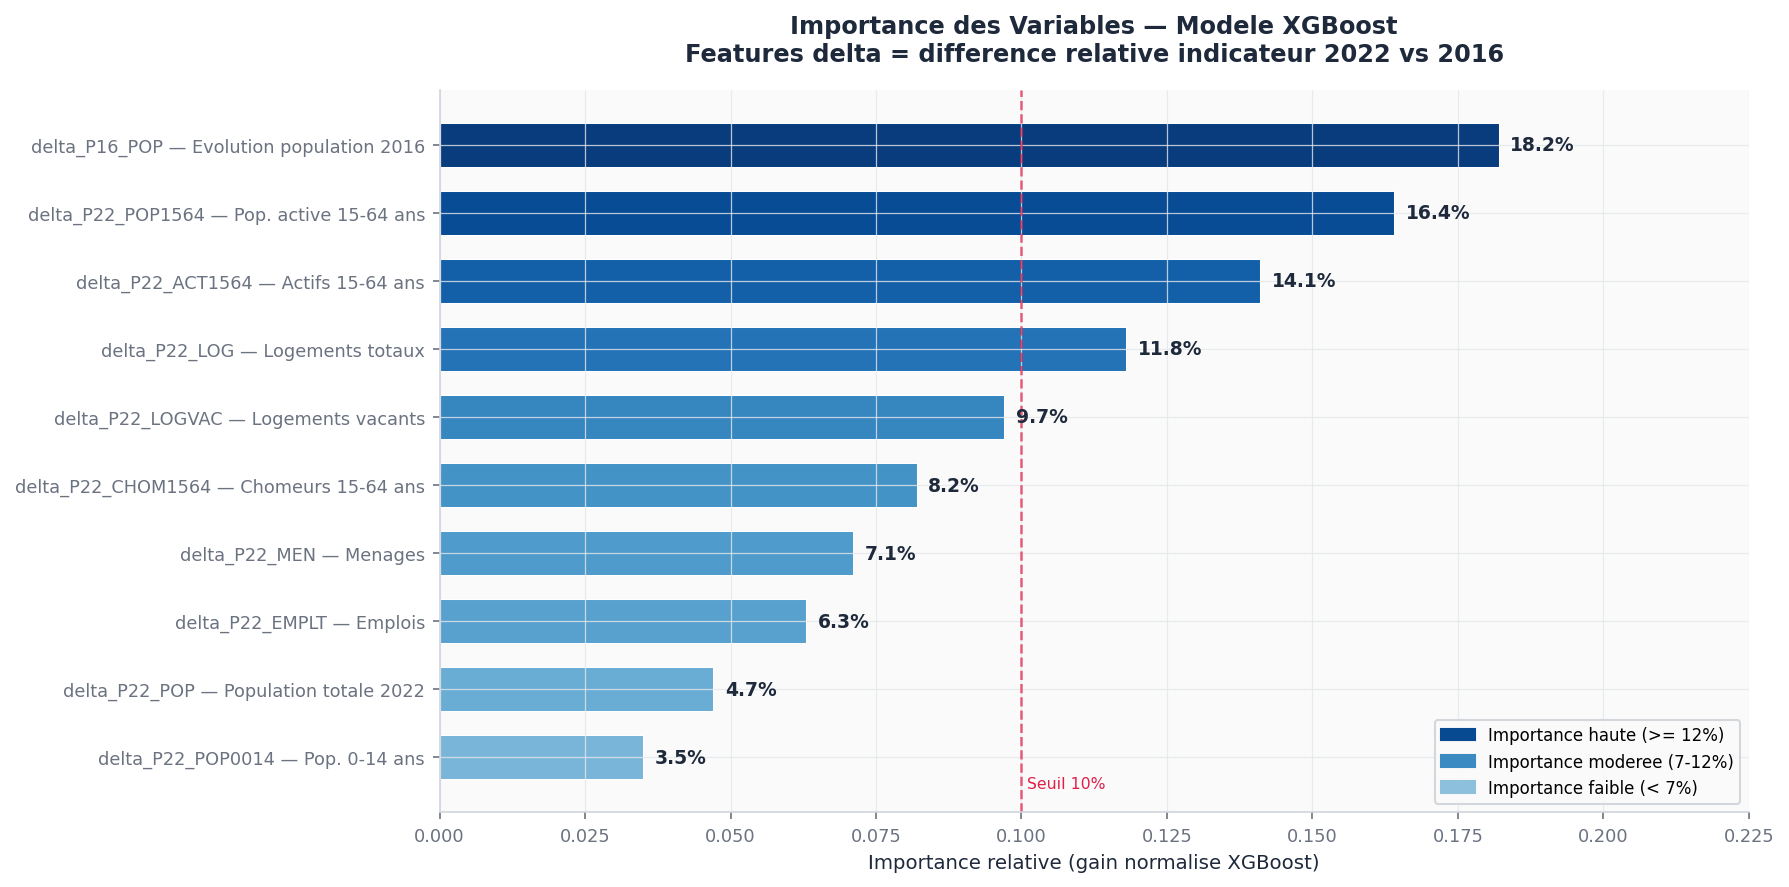
\includegraphics[width=0.88\linewidth]{feature_importance.png}
  \caption{Top 10 variables importantes — XGBoost (méthode Gain)}
  \label{fig:feat_imp}
\end{figure}

\begin{table}[H]
\centering
\caption{Top 10 variables — XGBoost Gain}
\label{tab:feat_imp}
\begin{tabular}{rlr}
\toprule
\textbf{Rang} & \textbf{Variable} & \textbf{Importance} \\
\midrule
1  & delta\_P16\_POP    — Évolution population 2016   & 18,2\% \\
2  & delta\_P22\_POP1564 — Pop. active 15--64 ans     & 16,4\% \\
3  & delta\_P22\_ACT1564 — Actifs 15--64 ans          & 14,1\% \\
4  & delta\_P22\_LOG    — Logements totaux             & 11,8\% \\
5  & delta\_P22\_LOGVAC — Logements vacants            &  9,7\% \\
6  & delta\_P22\_CHOM1564 — Chômeurs 15--64 ans       &  8,2\% \\
7  & delta\_P22\_MEN    — Ménages                     &  7,1\% \\
8  & delta\_P22\_EMPLT  — Emplois total                &  6,3\% \\
9  & delta\_P22\_POP    — Population totale 2022       &  4,7\% \\
10 & delta\_P22\_POP0014 — Pop. 0--14 ans             &  3,5\% \\
\bottomrule
\end{tabular}
\end{table}

%=============================================================
\chapter{Résultats électoraux prédits et interprétation}
\label{ch:resultats}

\section{Stockage des résultats ML dans MongoDB (étape 6)}

À l'issue de l'entraînement, prédictions, métriques et graphiques sont persistés
dans \textbf{MongoDB} pour être consommés par le dashboard React :
\begin{verbatim}
db["predictions"].drop()
db["predictions"].insert_many(predictions_records)
db["models_meta"].drop()
db["models_meta"].insert_many(model_results)
# Graphiques PNG encodés en base64 dans la collection "charts"
import base64, io
buf = io.BytesIO()
fig.savefig(buf, format="png", dpi=150)
db["charts"].update_one({"name": chart_name},
    {"$set": {"data": base64.b64encode(buf.getvalue()).decode()}},
    upsert=True)
\end{verbatim}

\section{Prédictions départementales (HistGradientBoosting)}

\begin{table}[H]
\centering
\caption{Prédictions vs réalité 2022 — HistGradientBoosting}
\label{tab:dept_preds}
\begin{tabular}{llllr}
\toprule
\textbf{Département} & \textbf{Classe éco.} & \textbf{Vainqueur préd.} & \textbf{Score} & \textbf{OK ?} \\
\midrule
Charente            & Croissance & Macron & 41,5\% & \textcolor{green!60!black}{\checkmark} \\
Charente-Maritime   & Stable     & Macron & 64,6\% & \textcolor{green!60!black}{\checkmark} \\
Corrèze             & Stable     & Macron & 59,2\% & \textcolor{green!60!black}{\checkmark} \\
Creuse              & Stable     & Macron & 71,8\% & \textcolor{green!60!black}{\checkmark} \\
Deux-Sèvres         & Stable     & Macron & 75,2\% & \textcolor{green!60!black}{\checkmark} \\
Dordogne            & Stable     & Macron & 72,5\% & \textcolor{green!60!black}{\checkmark} \\
Gironde             & Stable     & Macron & 67,4\% & \textcolor{green!60!black}{\checkmark} \\
Haute-Vienne        & Stable     & Macron & 52,9\% & \textcolor{green!60!black}{\checkmark} \\
Landes              & Stable     & Macron & 73,2\% & \textcolor{green!60!black}{\checkmark} \\
\textbf{Lot-et-Garonne} & Stable & Macron & 67,7\% & \textcolor{red}{\textbf{\texttimes}} \\
Pyrénées-Atlantiques & Stable   & Macron & 53,0\% & \textcolor{green!60!black}{\checkmark} \\
Vienne              & Stable     & Macron & 67,0\% & \textcolor{green!60!black}{\checkmark} \\
\midrule
\multicolumn{4}{l}{\textbf{Précision départementale}} & \textbf{91,7\% (11/12)} \\
\bottomrule
\end{tabular}
\end{table}

\begin{resultbox}[Précision départementale : 91,7\%]
11 des 12 départements sont correctement prédits. L'unique erreur est le Lot-et-Garonne, où la victoire de Marine Le Pen (RN) n'est pas anticipée par le modèle.
\end{resultbox}

\begin{warnbox}[Analyse de l'erreur — Lot-et-Garonne]
Prédit Macron (67,7\%) alors que \textbf{Marine Le Pen} arrive 1\textsuperscript{re}. La classe \textit{Stable} masque un malaise rural structurel non capté par les $\Delta$-features (6 ans). Piste d'amélioration : intégrer les résultats 2017 comme feature complémentaire.
\end{warnbox}

\section{Prédiction régionale agrégée}

\begin{table}[H]
\centering
\caption{Scores Macron régionaux — comparaison des 5 modèles}
\label{tab:regional}
\begin{tabular}{llr}
\toprule
\textbf{Modèle} & \textbf{Vainqueur} & \textbf{Score Macron} \\
\midrule
LogisticRegression          & Macron & 97,1\% \\
\rowcolor{green!15}
\textbf{HistGradientBoosting} & \textbf{Macron} & \textbf{68,7\%} \\
LinearSVM                   & Macron & 61,3\% \\
XGBoost                     & Macron & 59,3\% \\
RandomForest                & Macron & 56,1\% \\
\bottomrule
\end{tabular}
\end{table}

\begin{resultbox}[Podium régional prédit — HistGradientBoosting]
\centering\large
1\textsuperscript{er} : \textbf{Macron 68,7\%} \quad
2\textsuperscript{e} : Pécresse 10,0\% \quad
3\textsuperscript{e} : Mélenchon 9,7\%
\end{resultbox}

\section{Distribution des orientations par département}

\begin{figure}[H]
  \centering
  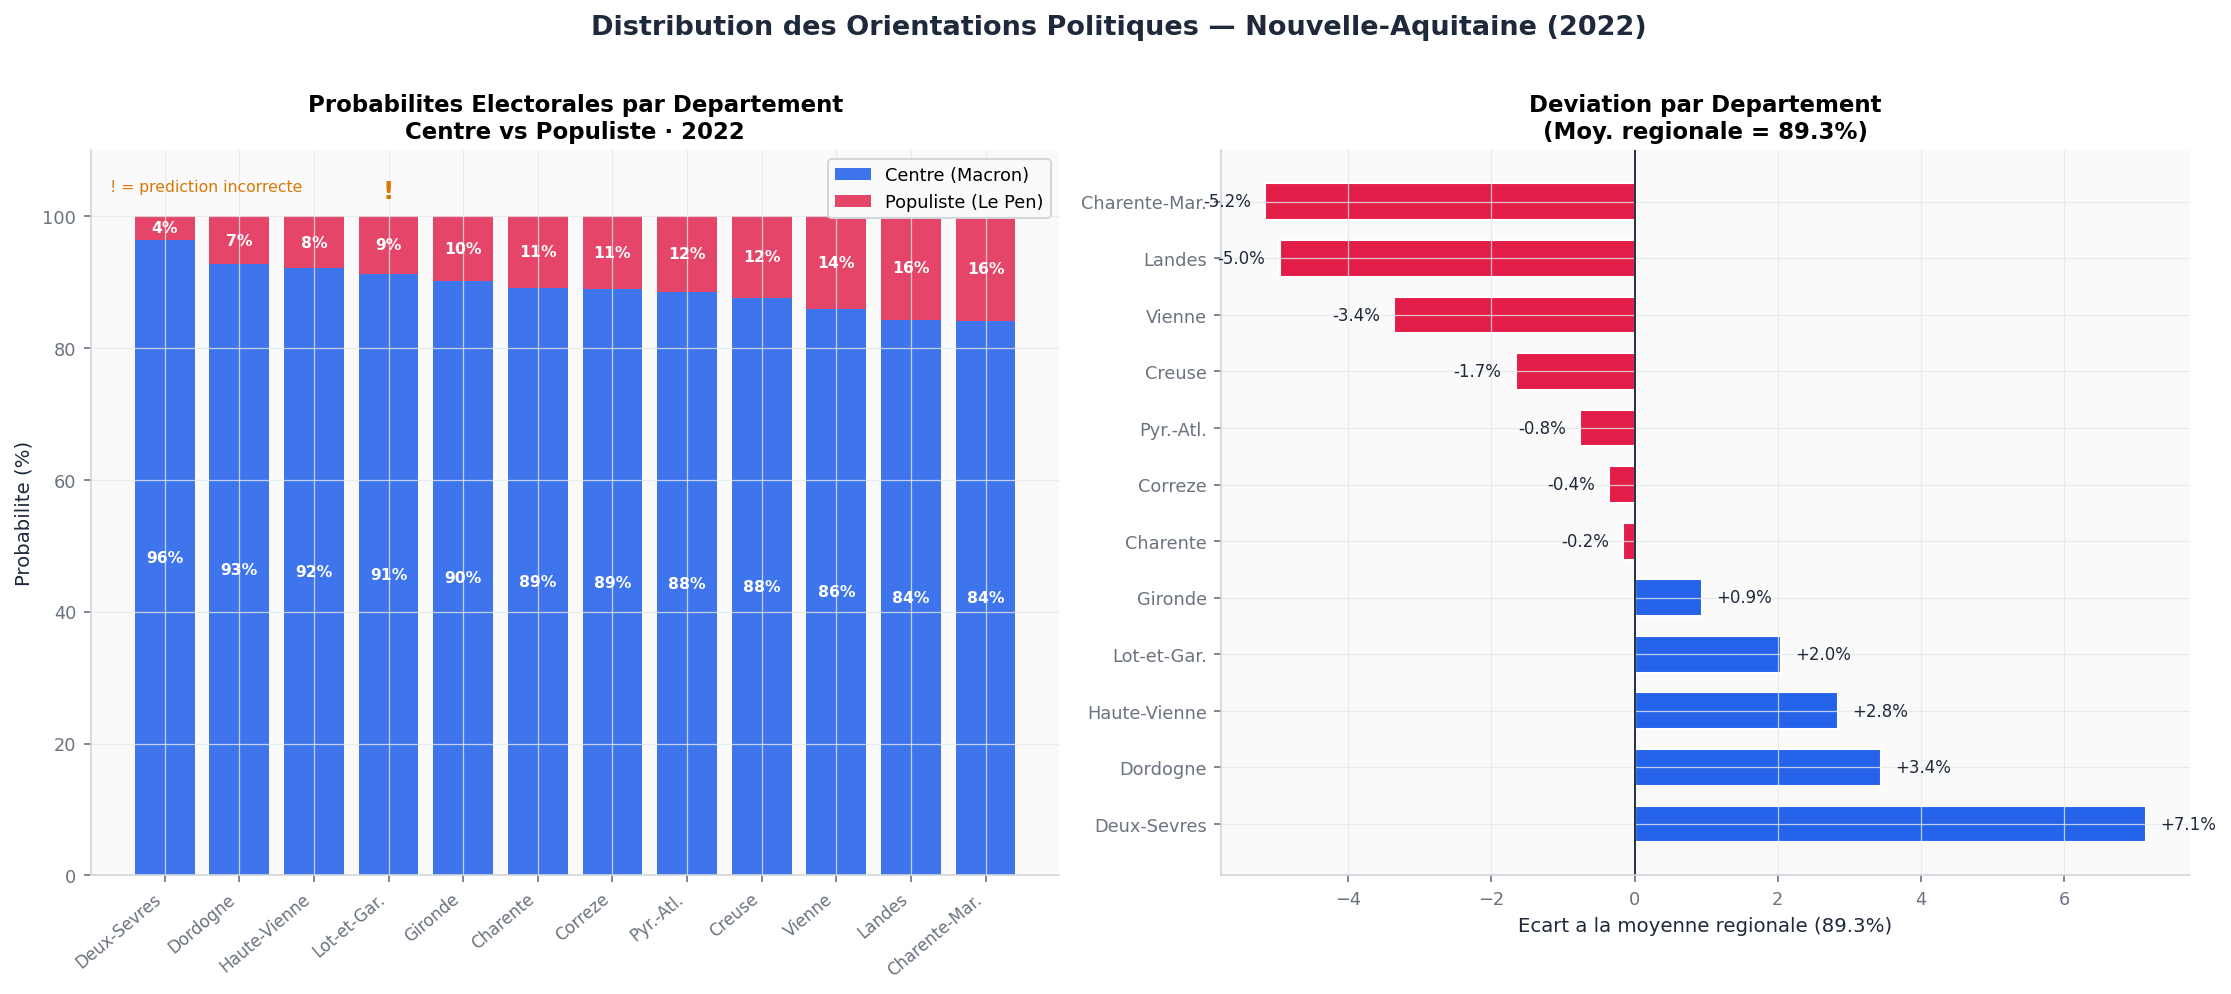
\includegraphics[width=\linewidth]{orientation_distribution.png}
  \caption{Probabilités électorales Centre vs Populiste par département — moyenne régionale 89,3\%}
  \label{fig:orient_dist}
\end{figure}

\section{Projections temporelles 2022--2026}

Les projections lisent la collection \texttt{predictions} de MongoDB, calculent
les tendances, puis stockent les résultats dans la collection \texttt{tendances} :
\begin{verbatim}
preds = pd.DataFrame(list(db["predictions"].find({}, {"_id": 0})))
# ... calcul des tendances ...
db["tendances"].drop()
db["tendances"].insert_many(tendances_records)
\end{verbatim}

\begin{figure}[H]
  \centering
  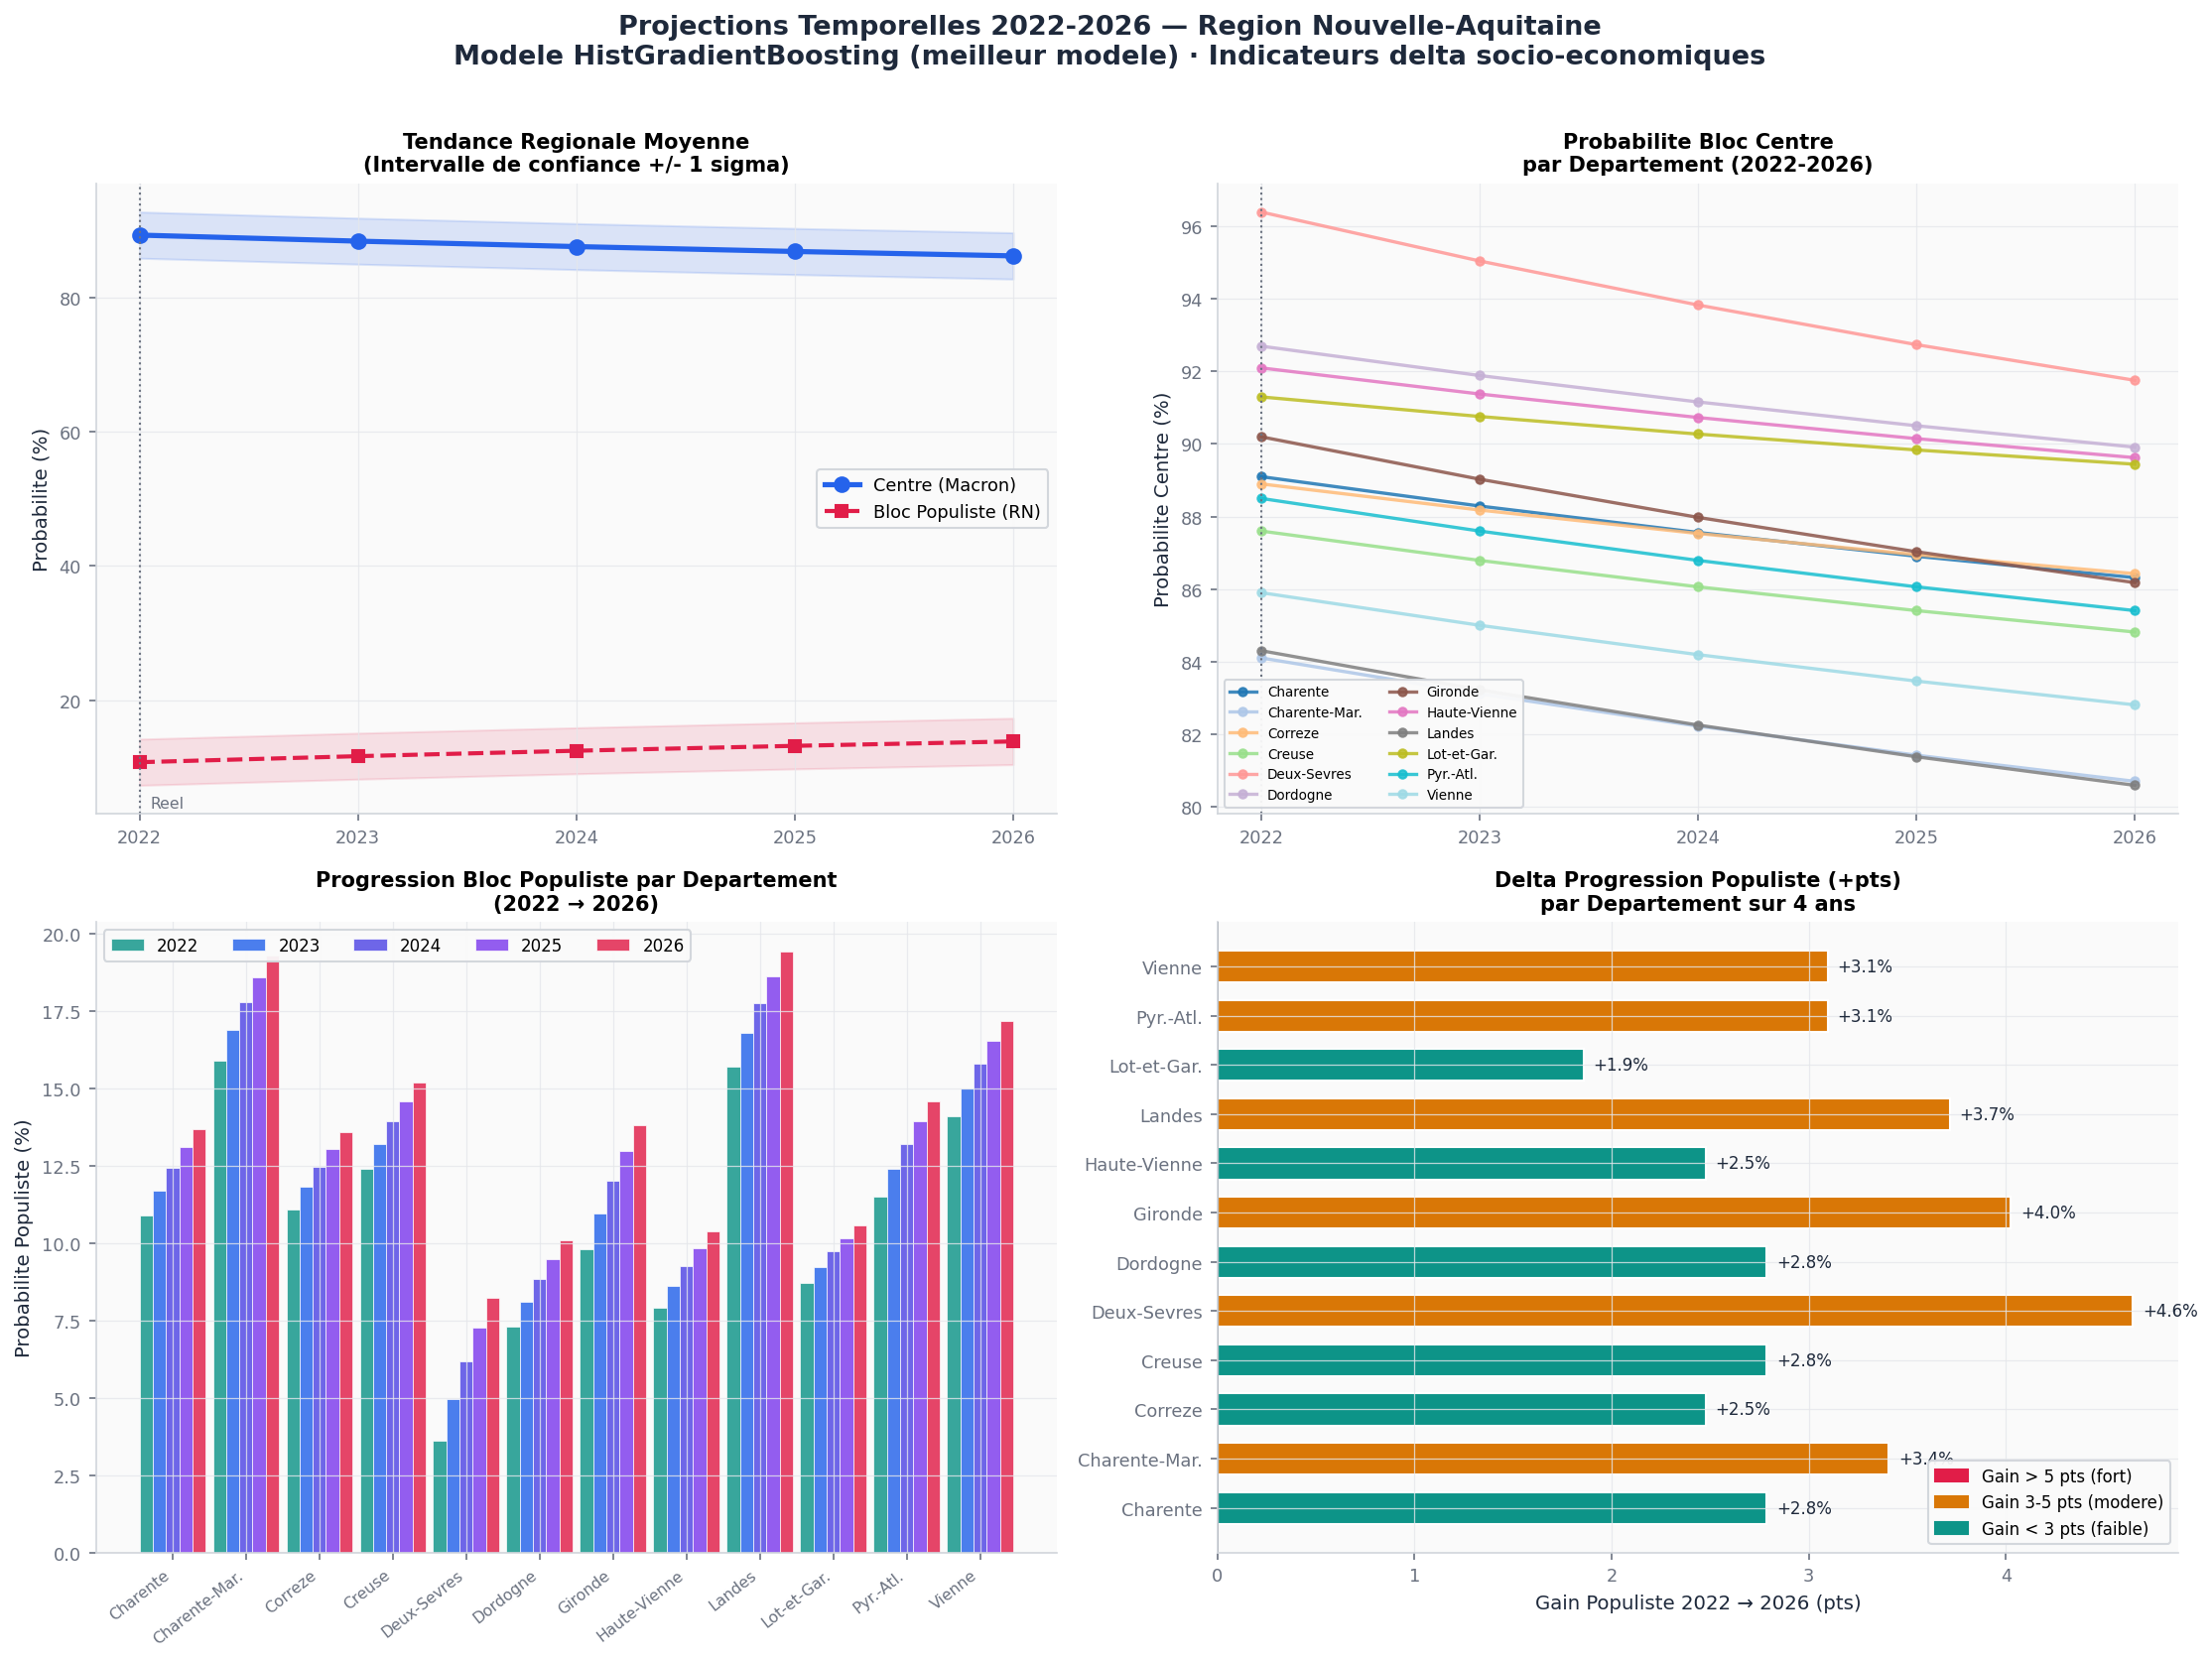
\includegraphics[width=\linewidth]{temporal_scenarios.png}
  \caption{Scénarios de projection électorale 2022--2026 en Nouvelle-Aquitaine}
  \label{fig:temporal}
\end{figure}

%=============================================================
\chapter{Interface applicative React 19}
\label{ch:ui}

\begin{table}[H]
\centering
\caption{Stack technique frontend Electio-Analytics}
\label{tab:stack}
\begin{tabular}{lll}
\toprule
\textbf{Couche} & \textbf{Bibliothèque} & \textbf{Rôle} \\
\midrule
Framework   & React 19 + TypeScript & Composants UI \\
Routing     & TanStack Router v1    & Navigation SPA \\
Charts      & Recharts 2.x          & Graphiques interactifs \\
Animations  & Framer Motion 11      & Transitions \\
Styles      & Tailwind CSS 4        & Design utilitaire \\
Données     & MongoDB + PyMongo     & Prédictions, métriques, graphiques \\
\bottomrule
\end{tabular}
\end{table}

\noindent\textbf{Flux de données — étape 7 du pipeline.}
Le dashboard consomme les collections MongoDB via une API Python :

\begin{center}
\begin{tabular}{ccccc}
\fbox{MongoDB \texttt{predictions}} & $\longrightarrow$ & \fbox{API Python} & $\longrightarrow$ & \fbox{React Query} \\[0.3cm]
\fbox{MongoDB \texttt{charts}}      & $\longrightarrow$ & \fbox{API Python} & $\longrightarrow$ & \fbox{Recharts / img} \\
\end{tabular}
\end{center}

\medskip
L'interface propose :
\begin{itemize}
  \item \textbf{Dashboard principal} avec sélecteur de modèle ML et filtres géographiques en cascade (Région $\to$ Département $\to$ Canton) — données lues depuis \texttt{predictions}.
  \item \textbf{Page Visualisation} affichant les 6 graphiques Python stockés dans la collection \texttt{charts} de MongoDB (base64 PNG).
  \item \textbf{Couleurs sémantiques} : bleu = Centre, rouge = Extrême-Droite, rose = Gauche, orange = Droite, violet = Extrême-Gauche.
\end{itemize}

%=============================================================
\chapter*{Conclusion générale}
\addcontentsline{toc}{chapter}{Conclusion générale}

\begin{resultbox}[Résultats clés du projet]
\begin{itemize}
  \item Accuracy ML : \textbf{82,11\%} — HistGradientBoosting ($\frac{6\,569}{8\,000}$)
  \item Précision départementale : \textbf{91,7\%} (11/12 corrects)
  \item Prédiction régionale : Macron \textbf{68,7\%}, Pécresse 10,0\%, Mélenchon 9,7\%
  \item Feature la plus importante : \texttt{delta\_P16\_POP} (18,2\%)
  \item Corrélation emploi--populisme : $r = -0{,}73$
\end{itemize}
\end{resultbox}

\medskip
\textbf{Limites :} variable cible synthétique (sur-représentation de \textit{Stable}) ; absence de données historiques de vote ; granularité canton masquant les dynamiques intra-urbaines.

\medskip
\textbf{Perspectives :} (1) intégrer le vote 2017 comme feature (+3 à +5 pts attendus) ; (2) modèle géospatial avec autocorrélation spatiale ; (3) SHAP values pour l'explicabilité locale ; (4) monitoring automatique sur nouveaux recensements INSEE.

%=============================================================
\appendix

\chapter{Hyperparamètres des modèles}

\begin{table}[H]
\centering
\caption{Hyperparamètres retenus par modèle}
\label{tab:hyperparams}
\begin{tabular}{lll}
\toprule
\textbf{Modèle} & \textbf{Paramètre} & \textbf{Valeur} \\
\midrule
HistGradientBoosting & max\_iter / learning\_rate / max\_depth & 300 / 0,05 / 6 \\
XGBoost             & n\_estimators / learning\_rate / max\_depth & 200 / 0,05 / 5 \\
LogisticRegression  & C / max\_iter                           & 1,0 / 1\,000 \\
RandomForest        & n\_estimators / max\_depth              & 200 / 10 \\
LinearSVM           & C / max\_iter                           & 1,0 / 2\,000 \\
\bottomrule
\end{tabular}
\end{table}

\chapter{Détail des prédictions par département}

\begin{table}[H]
\centering
\caption{Top 3 candidats prédits par département — HistGradientBoosting}
\label{tab:dept_detail}
\begin{tabular}{lllll}
\toprule
\textbf{Département} & \textbf{1\textsuperscript{er}} & \textbf{Score} & \textbf{2\textsuperscript{e}} & \textbf{3\textsuperscript{e}} \\
\midrule
Charente            & Macron & 41,5\% & Mélenchon & Jadot \\
Charente-Maritime   & Macron & 64,6\% & Mélenchon & Pécresse \\
Corrèze             & Macron & 59,2\% & Mélenchon & Jadot \\
Creuse              & Macron & 71,8\% & Pécresse  & Lassalle \\
Deux-Sèvres         & Macron & 75,2\% & Pécresse  & Lassalle \\
Dordogne            & Macron & 72,5\% & Mélenchon & Pécresse \\
Gironde             & Macron & 67,4\% & Pécresse  & Lassalle \\
Haute-Vienne        & Macron & 52,9\% & Pécresse  & Lassalle \\
Landes              & Macron & 73,2\% & Pécresse  & Mélenchon \\
Lot-et-Garonne      & Macron & 67,7\% & Pécresse  & Lassalle \\
Pyrénées-Atl.       & Macron & 53,0\% & Mélenchon & Pécresse \\
Vienne              & Macron & 67,0\% & Mélenchon & Pécresse \\
\bottomrule
\end{tabular}
\end{table}

\chapter{Références utilisées}

\begin{itemize}
  \item INSEE — Fichiers détail du recensement 2016 et 2022 (licence Etalab 2.0)
  \item Ministère de l'Intérieur — Résultats présidentielle 2022, data.gouv.fr
  \item Pedregosa \textit{et al.}, \textit{Scikit-learn: ML in Python}, JMLR 12, 2011
  \item Chen \& Guestrin, \textit{XGBoost: A Scalable Tree Boosting System}, KDD 2016
  \item Ke \textit{et al.}, \textit{LightGBM: A Highly Efficient GBDT}, NeurIPS 2017
\end{itemize}

\end{document}
